\documentclass[UTF8]{ctexart}

\usepackage{subfiles}  

%下面的语句, 引入你的头部设置文件
\usepackage{C:/phpStorm_proj/02_myself_ID_EGO/+100_latex_all_math_sel/myPreamble} 
%必须是绝对路径,才能让各个tex在单独编译时使用到

\title{文件名}


%---------------------------------


\begin{document}
	\tableofcontents % 生成目录
	\date{} % 若不写这句, 则默认也会渲染出日期, 所以我们要手动赋空值
	\maketitle  %这行代码, 让你前面的 title, author, date生效
	
	
	
	
	
	\part{全概率公式 : \\ $
		P\left( B \right) =\underbrace{P\left( A_1 \right) \cdot P\left( B|A_1 \right) }+\underbrace{P\left( A_2 \right) \cdot P\left( B|A_2 \right) }+...+\underbrace{P\left( A_n \right) \cdot P\left( B|A_n \right) }
$}
	
	全概率公式 Total Probability Theorem: \\	
	如果 $A_1, A_2, ..., A_n$ 构成一个``完备事件组", 即: (1) 这些事件两两互不相容,  (2)其``和"(或``并集")为全集 $\Omega$, (3) $P(A_i)>0$. \\
	
	则有:
	$\boxed{
		\sum_{i=1}^n{\,\,\left[ P\left( A_i \right) \cdot P\left( B|A_i \right) \right]}=P\left( B \right) 
	}
	$ \\
	
	
	即有: $
	P\left( B \right) =\underbrace{P\left( A_1 \right) \cdot P\left( B|A_1 \right) }+\underbrace{P\left( A_2 \right) \cdot P\left( B|A_2 \right) }+...+\underbrace{P\left( A_n \right) \cdot P\left( B|A_n \right) }
	$ \\
	
	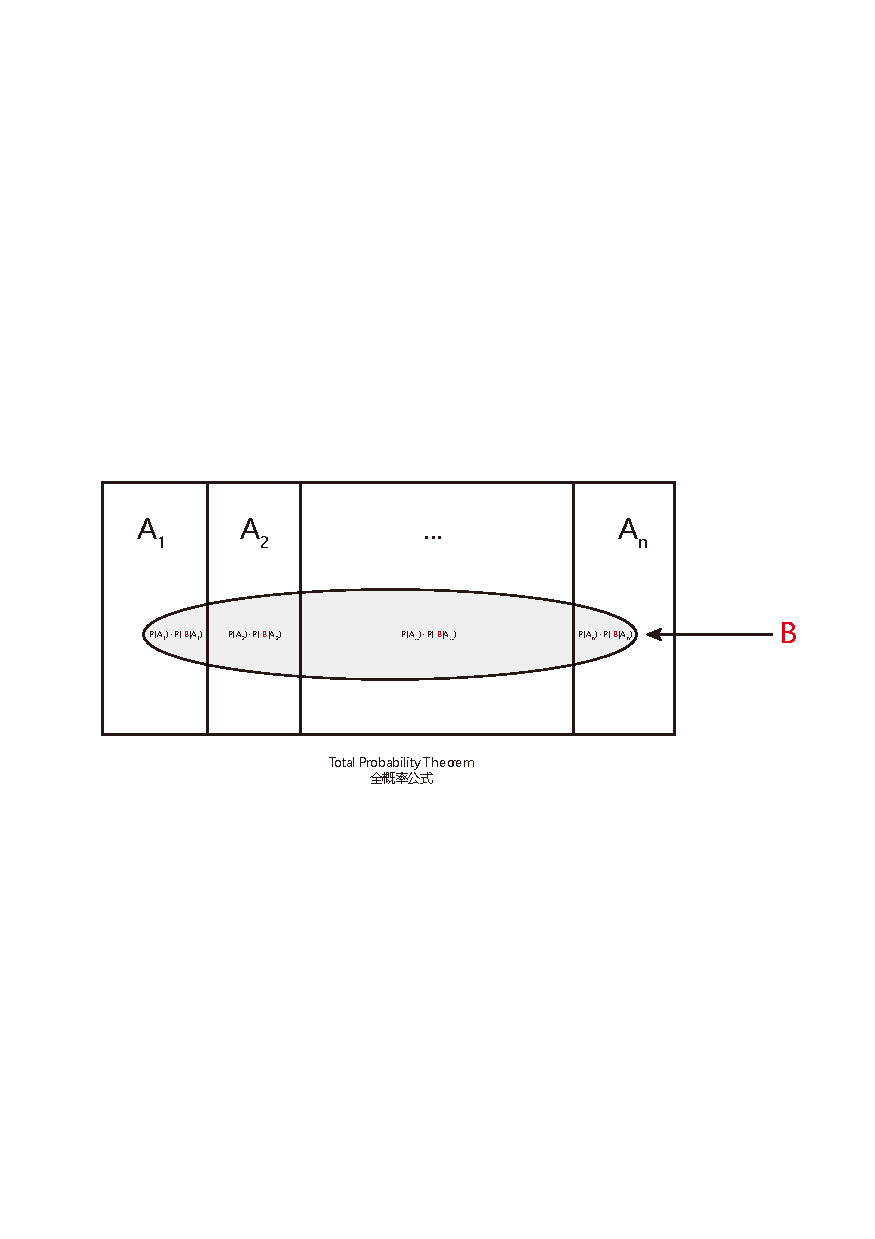
\includegraphics[width=1\textwidth]{/0095.pdf} \\
	
	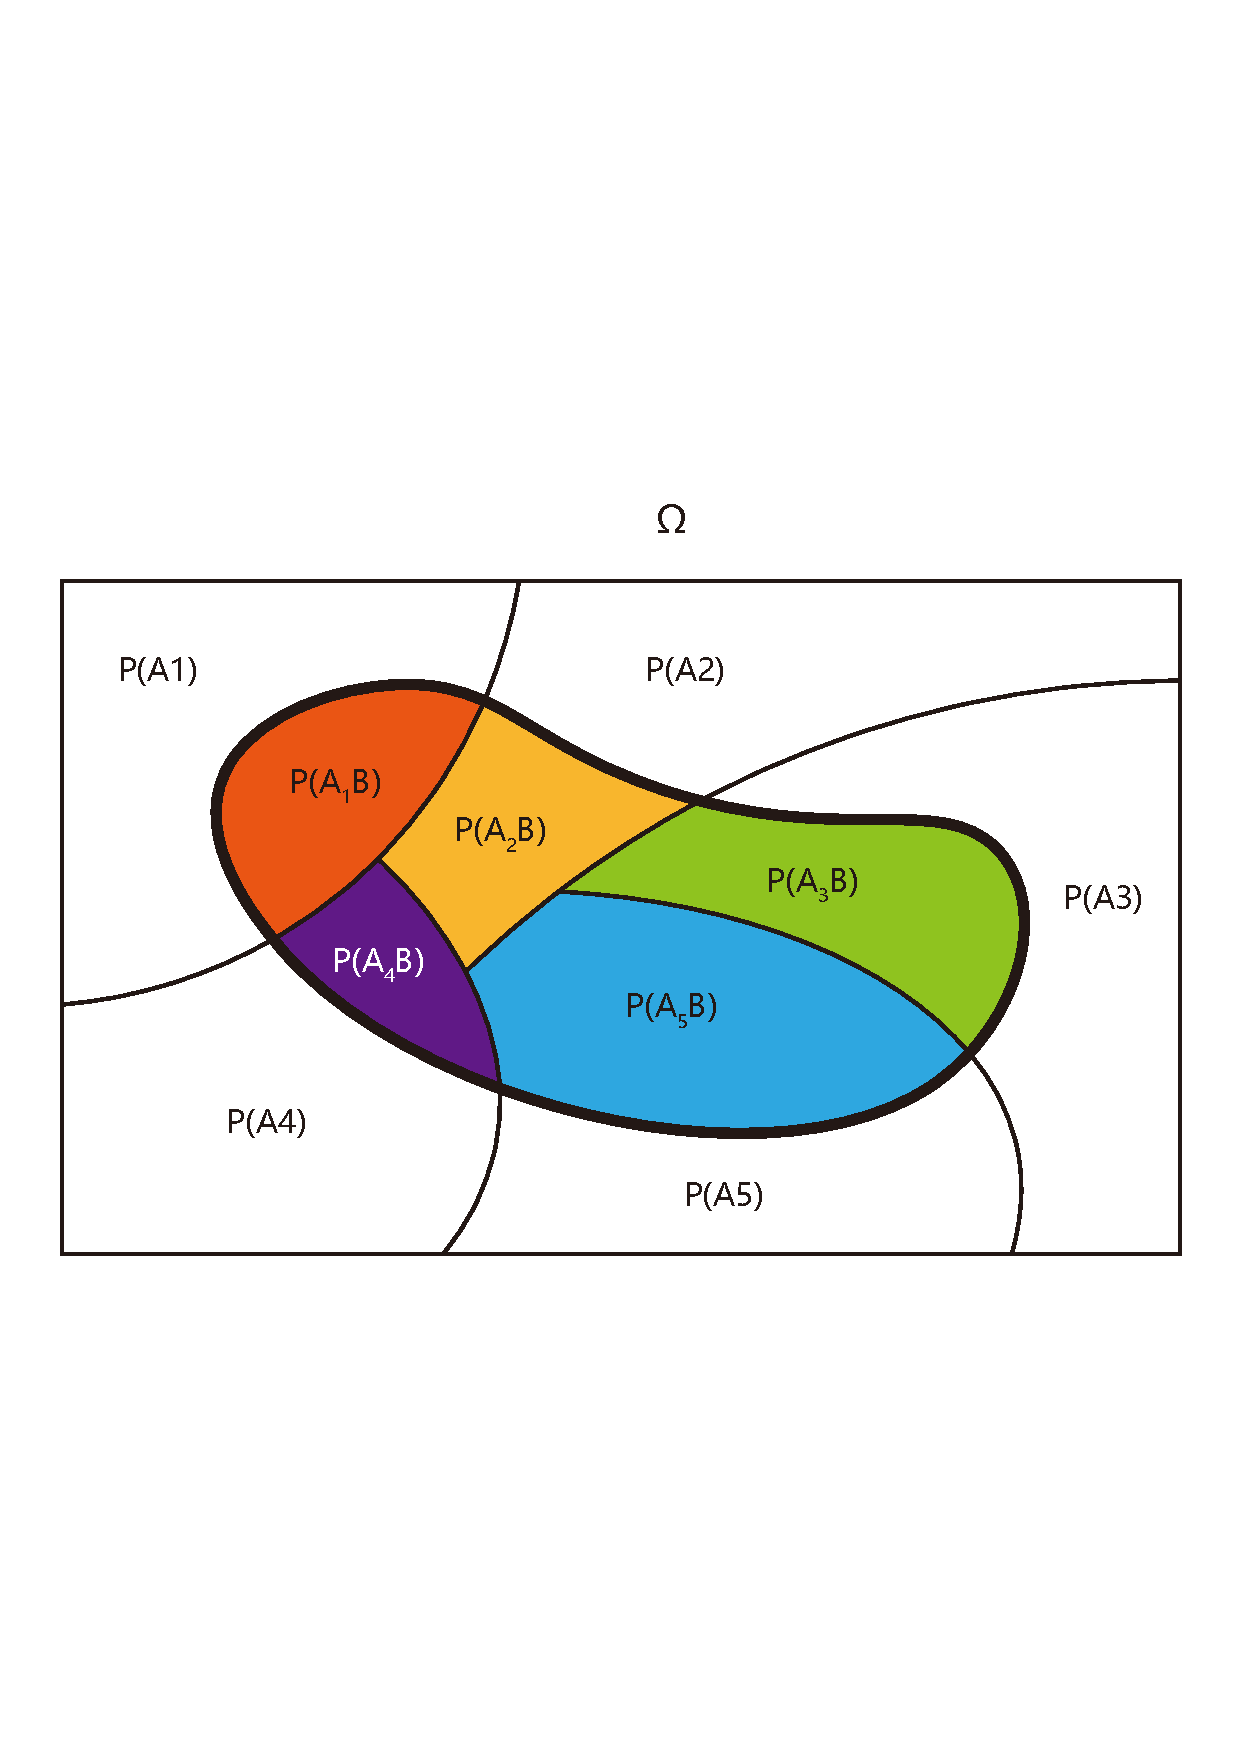
\includegraphics[width=0.6\textwidth]{/0105.pdf} \\
	
	上图, 粗线部分围起来的整块有彩色区域, 就是B.  \\
	B的概率, 就等于= 每一个彩色块的概率, 加总起来. \\
	
	比如第1块, 橙色的概率, 就是 A1 和 B 的交集, 即 $ = P(A_1 \cap B)$ \\
	P(B) = 所有5块彩色的概率 加起来. 即得到下图中的``全概率公式". \\
	
	全概率公式 : 
	\begin{align*}  % 支持每行编号. 若不需要编号, 就用 align*环境
		P\left( B \right) &=\text{第1块的概率}+\text{第2块的概率}+...+\text{第}n\text{块的概率}\\
		&=P\left( A_1B \right) +P\left( A_2B \right) +...+P\left( A_nB \right)\\
		&=P\left( A_1 \right) \cdot P\left( B|A_1 \right) +P\left( A_2 \right) \cdot P\left( B|A_2 \right) +...+P\left( A_n \right) \cdot P\left( B|A_n \right)\\
		&=\sum_{i=1}^n{\left[ P\left( A_i \right) \cdot P\left( B|A_i \right) \right]} 
	\end{align*}
	
	并有: $
	P\left( B \right) =\underset{A\text{中,}B\text{的概率的具体值}}{\underbrace{P\left( A \right) \cdot P\left( B|A \right) }}+\underset{}{\underbrace{P\left( \overline{A} \right) \cdot P\left( B|\overline{A} \right) }}
	$ \\
	
	注意: 上式中,  P(B|A) 这块只是个比例而已. 即 B在A中的比例. 即 $\frac{B} {A}$. 但单纯的比例是没用的. 比如, alice说她的收入只有 bob 的 1/10, 但 1/10 依然没有告诉你 alice的收入到底是多少? 所以, 比例值还需要乘上一个基数. 这个``基数"就是 bob 本身的收入, 比如是 10000元, 你才能知道 alice的收入是 $10000 \cdot \frac{1} {10} = 1000$元. \\
	
	同理, 本处的公式, P(B|A) 这个比例, 还要乘上``P(A) 本身的值"作为基数, 我们才能最终知道 P(AB)的具体值到底是多少. \\
	事实上, P(B|A) 就是 B占A的比例. 即 $\frac{B} {A}$. \\
	而 $P(A) \cdot  P(B|A)$ 就是 AB 的交集面积 占整个全集$\varOmega $ 的比例, 即$	\frac{A\cap B}{\varOmega}	$ \\
	
	如果我们把 全集分为 两部分: A 和 $ \overline{A}$, 则, B的部分, 就是: 
	\begin{align*}  % 支持每行编号. 若不需要编号, 就用 align*环境
		\boxed{
			P(B)= P(A) \cdot P(B |A) +  P( \overline{A}) \cdot P(B | \overline{A})
		}  
	\end{align*}
	
	如下图: \\
	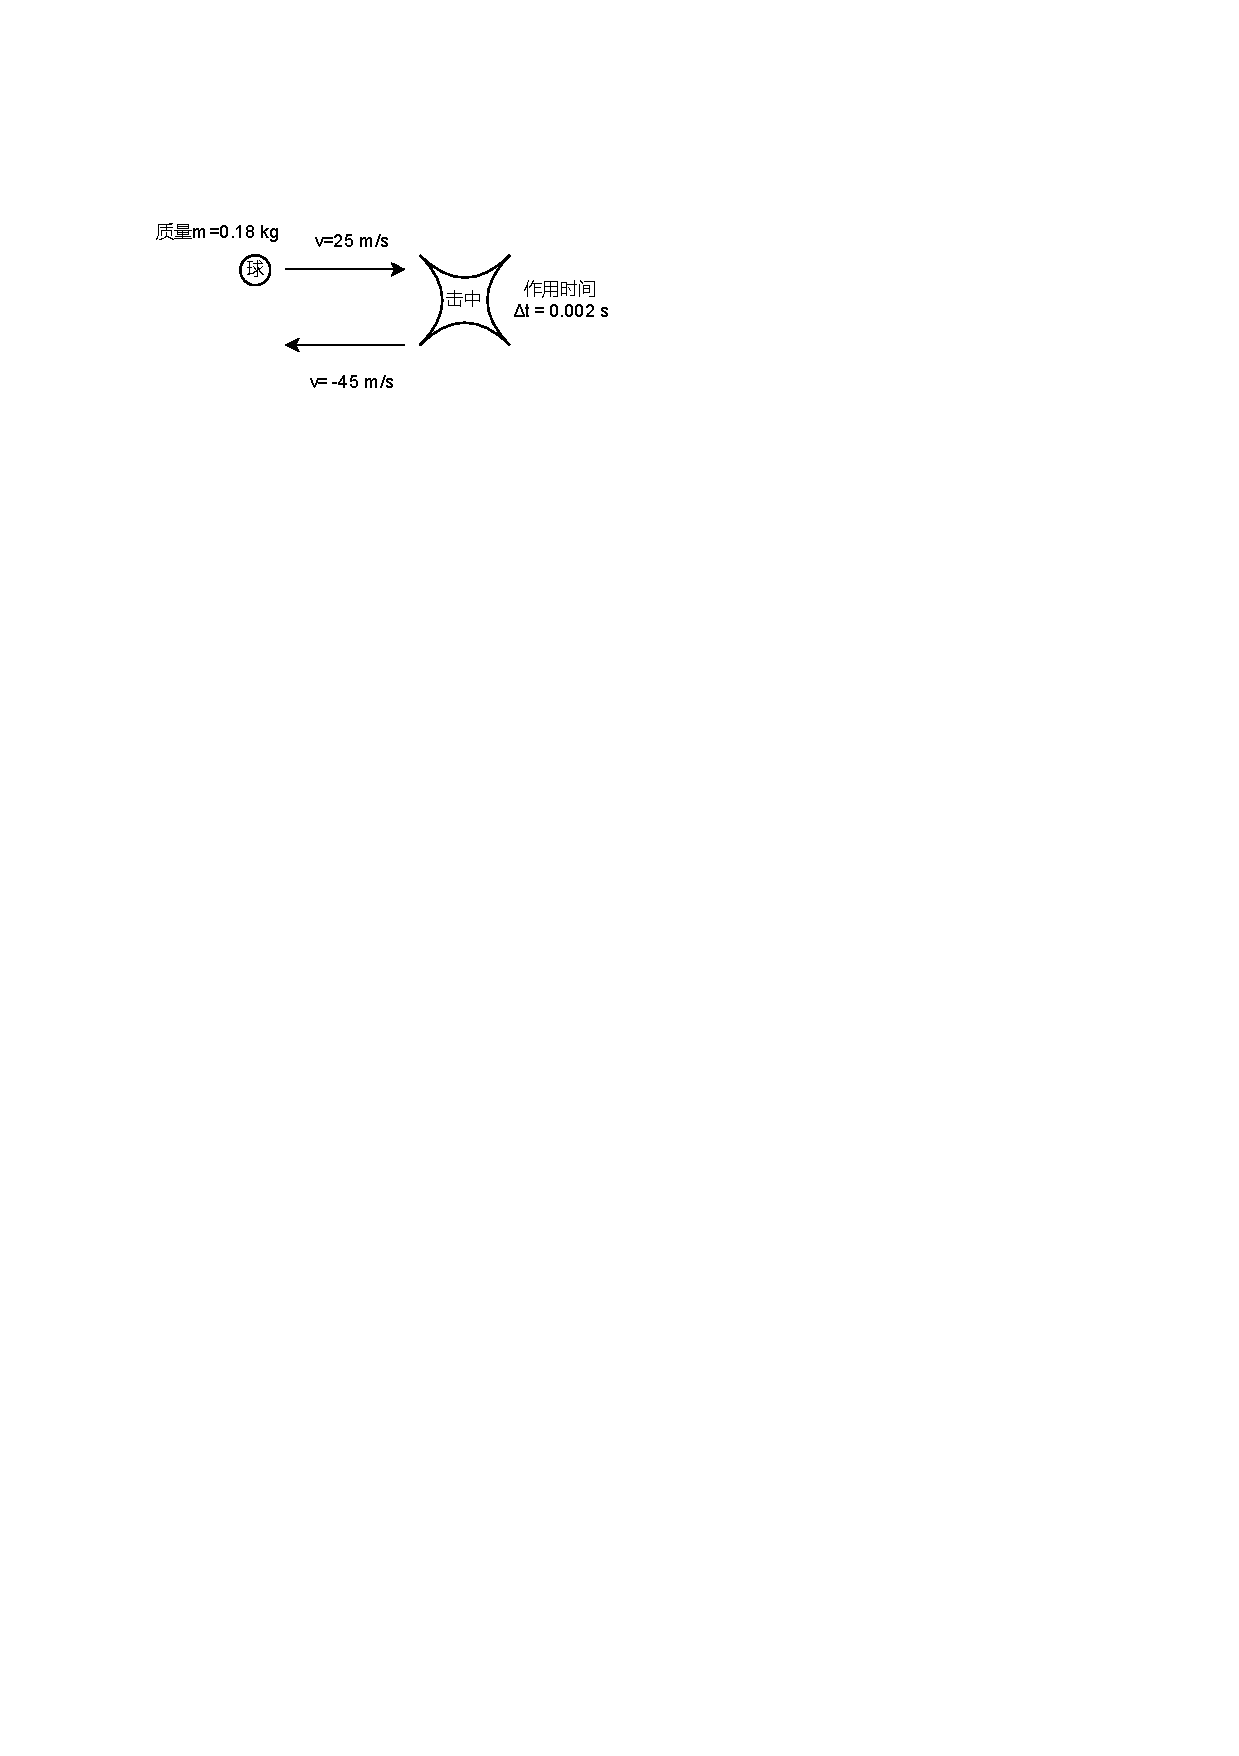
\includegraphics[width=0.5\textwidth]{/0106.pdf}
	
	比如, 全集 Ω (亚欧板块)被分成两部分: 一块是A(亚洲), 另一块是$\overline{A}$ (欧洲). 全集中有子集B(俄罗斯), 被A 和$\overline{A}$各自分割了一部分土地. 那么: 
	\begin{align*}  % 支持每行编号. 若不需要编号, 就用 align*环境
		\begin{matrix}
			\underset{\text{俄罗斯占亚欧板块的面积比例}}{\underbrace{P\left( B \right) }}
			&=\underset{\text{亚洲占亚欧板块的比例}}{\underbrace{P\left( A \right) }}\cdot \underset{\text{亚洲中的俄罗斯部分,占亚洲的比例}}{\underbrace{P\left( B|A \right) }}\\
			& +\underset{\text{欧洲占亚欧板块的比例}}{\underbrace{P\left( \overline{A} \right) }}\cdot \underset{\text{欧洲中的俄罗斯部分,占欧洲的比例}}{\underbrace{P\left( B|\overline{A} \right) }}\\
		\end{matrix}
	\end{align*}
	
	
	
	
	
	
	
	\begin{myEnvSample}
		一个工厂, 有4条生产线, 情况如下: \\	
		\begin{tabular}{|l| l| l| l| l|}
			\hline
			&  生产线1  & 生产线2  &  生产线3 & 生产线4 \\
			\hline
			产量 &  15\% & 20\% & 30\% & 35\% \\
			\hline
			不合格率 &  0.05 & 0.04 & 0.03 & 0.02 \\
			\hline
		\end{tabular} \\
		
		问: 从该工厂的产品中, 任取一件, 是``不合格品"的概率? \\
		
		我们先设定事件: \\
		- $A_1$ : 表示是 生产线1 中的产品 \\
		- $A_2$ : 表示是 生产线2 中的产品 \\
		- $A_3$ : 表示是 生产线3 中的产品 \\
		- $A_4$ : 表示是 生产线4 中的产品 \\
		- $B$ : 表示是次品 \\
		
		那么, 你任取一件为不合格的概率, 不就是整个工厂总的不合格概率么?! 即 =P(B) \\		
		\begin{align*}
			&P\left( B \right)\\
			&=\underset{\text{第1条生产线中}\left( \text{的条件下} \right) ,\,\,\text{不合格品的概率}}{\underbrace{\overset{\text{产品属于生产线1的概率}}{\overbrace{P\left( A_1 \right) }}\cdot \overset{\text{生产线1中的次品率}}{\overbrace{P\left( B|A_1 \right) }}}}+P\left( A_2 \right) \cdot P\left( B|A_2 \right) +P\left( A_3 \right) \cdot P\left( B|A_3 \right) +P\left( A_4 \right) \cdot P\left( B|A_4 \right)\\
			&=(15\%\cdot 0.05)+(20\%\cdot 0.04)+(30\%\cdot 0.03)+(35\%\cdot 0.02)\\
			&=0.0315
		\end{align*}
	\end{myEnvSample}
	\vspace{1em} 
	
	
	
	\begin{myEnvSample}
		有10台机器人, 3台是次品. 已经卖出去了2台(是正品还是次品未知). \\
		问: 再取1台, 是正品的概率? \\
		
		首先, 我们定义事件:  \\
		- $B_{00}$ : B(bad),  表示前两次取, 都是次品(用0表示) \\
		- $B_{10}$ : 表示前两次取, 是 一正(用1表示), 一次(用0表示). 至于顺序是``正,次" 还是``次,正", 都行 \\
		- $B_{11}$ : 表示前两次取, 都是正品 \\
		- $G_{xx3}$ : G(good),  表示第三次取, 是正品 \\
		
		那么, 第3次取到正品 $P(G_{xx3})$ 的情况, 就有这3种可能性: \\
		- (第1次取到)次, (第2次取到)次, (第4次取到)正.  \\
		即 → $=
		\underset{\text{前两次取到次品}}{\underbrace{\text{P}\left( \text{B}_{00} \right) }}\cdot \underset{\text{在前两次取到次品的条件下,\ 第3次取到正品}}{\underbrace{\text{P}\left( \text{G}_{\text{xx}3}\ |\text{B}_{00} \right) }}
		$ \\
		- 次,正,正.  即 → $=
		\text{P}\left( \text{B}_{10} \right) \cdot \text{P}\left( \text{G}_{\text{xx}3}\ |\text{B}_{10} \right) 
		$ \\
		- 正,正,正. 即 →  $=
		\text{P}\left( \text{B}_{11} \right) \cdot \text{P}\left( \text{G}_{\text{xx}3}\ |\text{B}_{11} \right) 
		$\\
		
		上面这三种可能性并存, 就是``和"(并集)的概念. 用加法: \\
		
		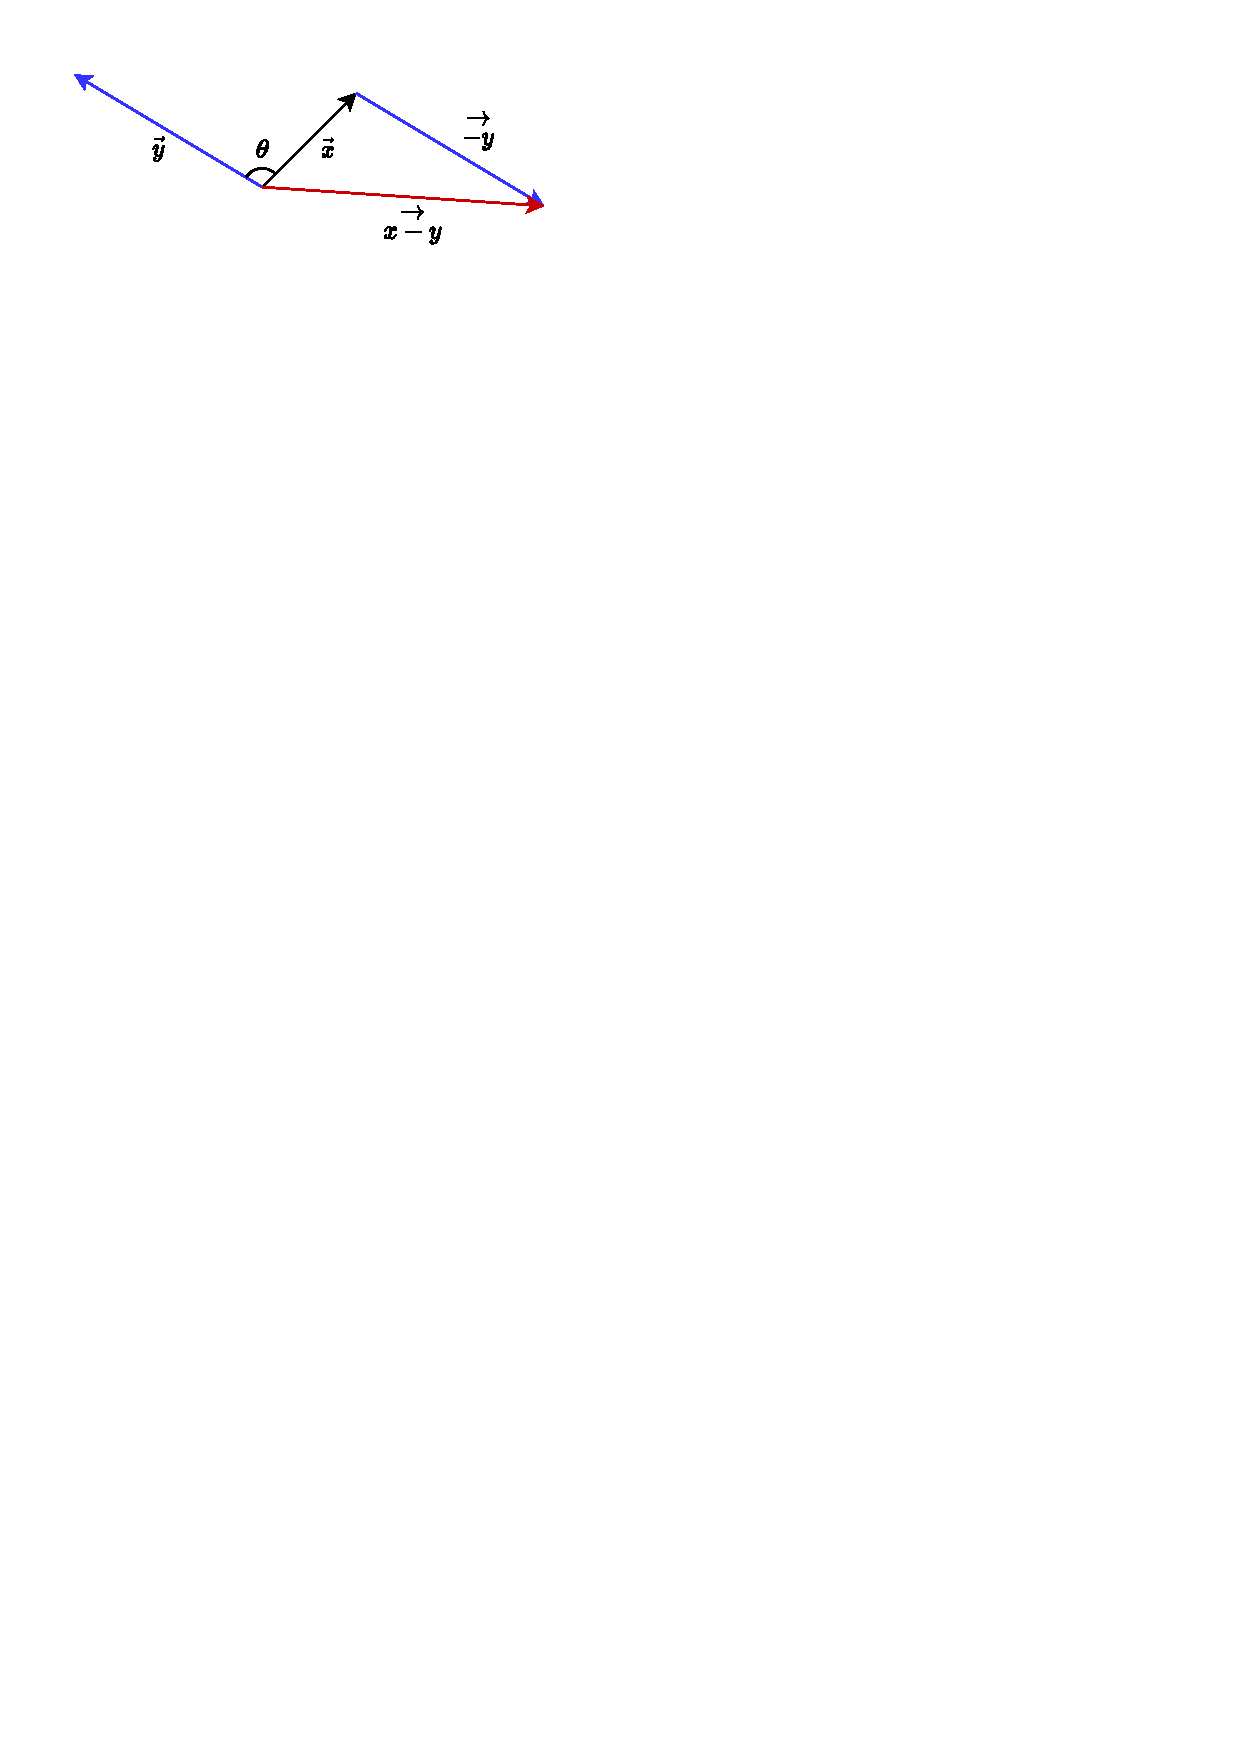
\includegraphics[width=1\textwidth]{/0096.pdf}
		
		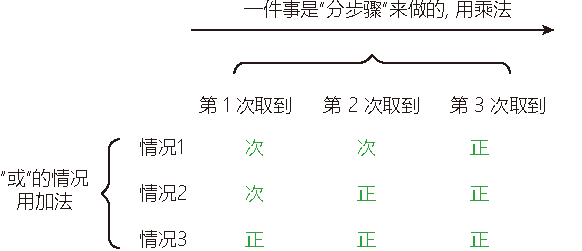
\includegraphics[width=0.7\textwidth]{/0097.pdf}
	\end{myEnvSample}
	\vspace{1em} 
	
	
	
	
	\begin{myEnvSample}
		有10件产品, 其中次品的数量, 有三种可能性: 0件 /1件 /2件, 即这三种可能性中的每一种, 发生的概率是1/3.  \\
		同时, 检验时也存在``误检"情况 : \\
		\begin{tabular}{|l|l|l|l|}
			\hline
			& →被检验成→ &    & 的概率是   \\
			\hline
			正品 &        & 次品 & 0.02    \\
			\hline
			正品 &    →    & 正品 & 0.98    \\
			\hline
			次品 &   →     & 正品 & 0.05    \\
			\hline
			次品 &        & 次品 & 0.96  \\
			\hline
		\end{tabular}\\
		
		问: 这批产品能通过检验(即事件$S_2$)的可能性是多少? 即本题要求 P($S_2$)=? \\
		这要分两种情况来讨论 (``和"的概念, 用加法): \\
		- 1. 正品被误检(成``假")时的情况 \\
		- 2. 次品被误检(成``真")时的情况 \\
		
		我们先定义各种事件: \\
		- $B_0$ : B(bad). 表示总的10件产品中, 存在0件次品. 该事件的概率, 题目已经告诉我们: $\text{P}\left( \text{B}_0 \right) =\frac{1}{3}$
		\\
		- $B_1$ : 表示总的10件产品中, 存在1件次品. $\text{P}\left( \text{B}_1 \right) =\frac{1}{3}$
		\\
		- $B_2$ : 表示总的10件产品中, 存在2件次品. $\text{P}\left( \text{B}_2 \right) =\frac{1}{3}$
		\\
		- $S_1$ : S(sample. (v.) 抽样检验;取样;采样) 表示任意抽检一次, 抽到了正品. (但这里还有个问题不清晰, 就是说这个正品, 到底是它本身就是``正品"; 还是说只是抽验认为它是``正品"?) \\
		- $\overline{S_1}$ : 表示任意抽检一次, 抽到了次品. \\
		- $S_2$ : 表示再次检验, 并``通过验证" (注意: 有误检率存在. 所以通过检验的, 未必是``正品"; 反之亦然). \\
		
		
		本题要求的 P($S_2$), 实际上就是: ``无论第一次抽, 认为是正是次; 在第二次检验时, 都认为是正品"的东西. 即: $
		\text{P}\left( \text{S}_2 \right) =\underset{\text{第一次抽为正品,第二次检验为正}}{\underbrace{\text{P}\left( \text{S}_1 \right) \cdot \text{P}\left( \text{S}_2\ |\text{S}_1 \right) }}+\underset{\text{第一次抽为次品,第二次检验为正}}{\underbrace{\text{P}\left( \overline{\text{S}_1} \right) \cdot \text{P}\left( \text{S}_2\ |\overline{\text{S}_1} \right) }}
		$ \\
		
		那么我们先考算 $	\text{P}\left( \text{S}_1 \right) 	$ 和	$	\text{P}\left( \overline{\text{S}_1} \right) 	$. \\
		
		→ $	\text{P}\left( \text{S}_1 \right) 	$ : 是在具体``次品"数量未知的情况下, 抽1次就得到``正品"的概率. \\
		\begin{align*}  % 支持每行编号. 若不需要编号, 就用 align*环境
			&	\text{P}\left( \text{S}_1 \right) =\underset{\text{在总数中有0次品的条件下,\ 抽1次得到正品的概率}}{\underbrace{\overset{\text{总数中有0次品}}{\overbrace{\text{P}\left( \text{B}_0 \right) }}\cdot \text{P}\left( \overset{\text{第1次抽得到正品}}{\overbrace{\text{S}_1}}|\text{B}_0 \right) }}+\underset{\text{总数中含有1次品,\ 抽1次取到正}}{\underbrace{\text{P}\left( \text{B}_1 \right) \cdot \text{P}\left( \text{S}_1|\text{B}_1 \right) }}+\underset{\text{总数中含有2次品,\ 抽1次取到正}}{\underbrace{\text{P}\left( \text{B}_2 \right) \cdot \text{P}\left( \text{S}_1|\text{B}_2 \right) }}\\
			&=\underset{\text{总10中含有0次品}}{\underbrace{\frac{1}{3}\cdot \frac{\text{C}_{\text{总10正}}^{1}}{\text{C}_{\text{总}10}^{1}}}}+\underset{\text{总10中含有1次品}}{\underbrace{\frac{1}{3}\cdot \frac{\text{C}_{\text{总9正}}^{1}}{\text{C}_{\text{总}10}^{1}}}}+\underset{\text{总10中含有2次品}}{\underbrace{\frac{1}{3}\cdot \frac{\text{C}_{\text{总8正}}^{1}}{\text{C}_{\text{总}10}^{1}}}}\\
			&=0.9  
		\end{align*} 	
		
		所以 : $
		\text{P}\left( \overline{\text{S}_1} \right) =1-\text{P}\left( \text{S}_1 \right) =1-0.9=0.1
		$ \\
		
		于是, 我们就能得到 : \\
		\begin{align*}  % 支持每行编号. 若不需要编号, 就用 align*环境
			&\text{P}\left( \text{S}_2 \right) =\underset{\text{第一次抽为正品,第二次检验为正}}{\underbrace{\overset{=0.9}{\overbrace{\text{P}\left( \text{S}_1 \right) }}\cdot \overset{\text{从上面的表格中可知,\ 正品被检验为正品,概率为}0.98}{\overbrace{\text{P}\left( \text{S}_2\ |\text{S}_1 \right) }}}}+\underset{\text{第一次抽为次品,第二次检验为正}}{\underbrace{\overset{=0.1}{\overbrace{\text{P}\left( \overline{\text{S}_1} \right) }}\cdot \overset{\text{次品被检验为正品,\ 概率是}0.05}{\overbrace{\text{P}\left( \text{S}_2\ |\overline{\text{S}_1} \right) }}}}\\
			&=\left( 0.9\cdot 0.98 \right) +\left( 0.1\cdot 0.05 \right) =0.887\\
		\end{align*}
		
		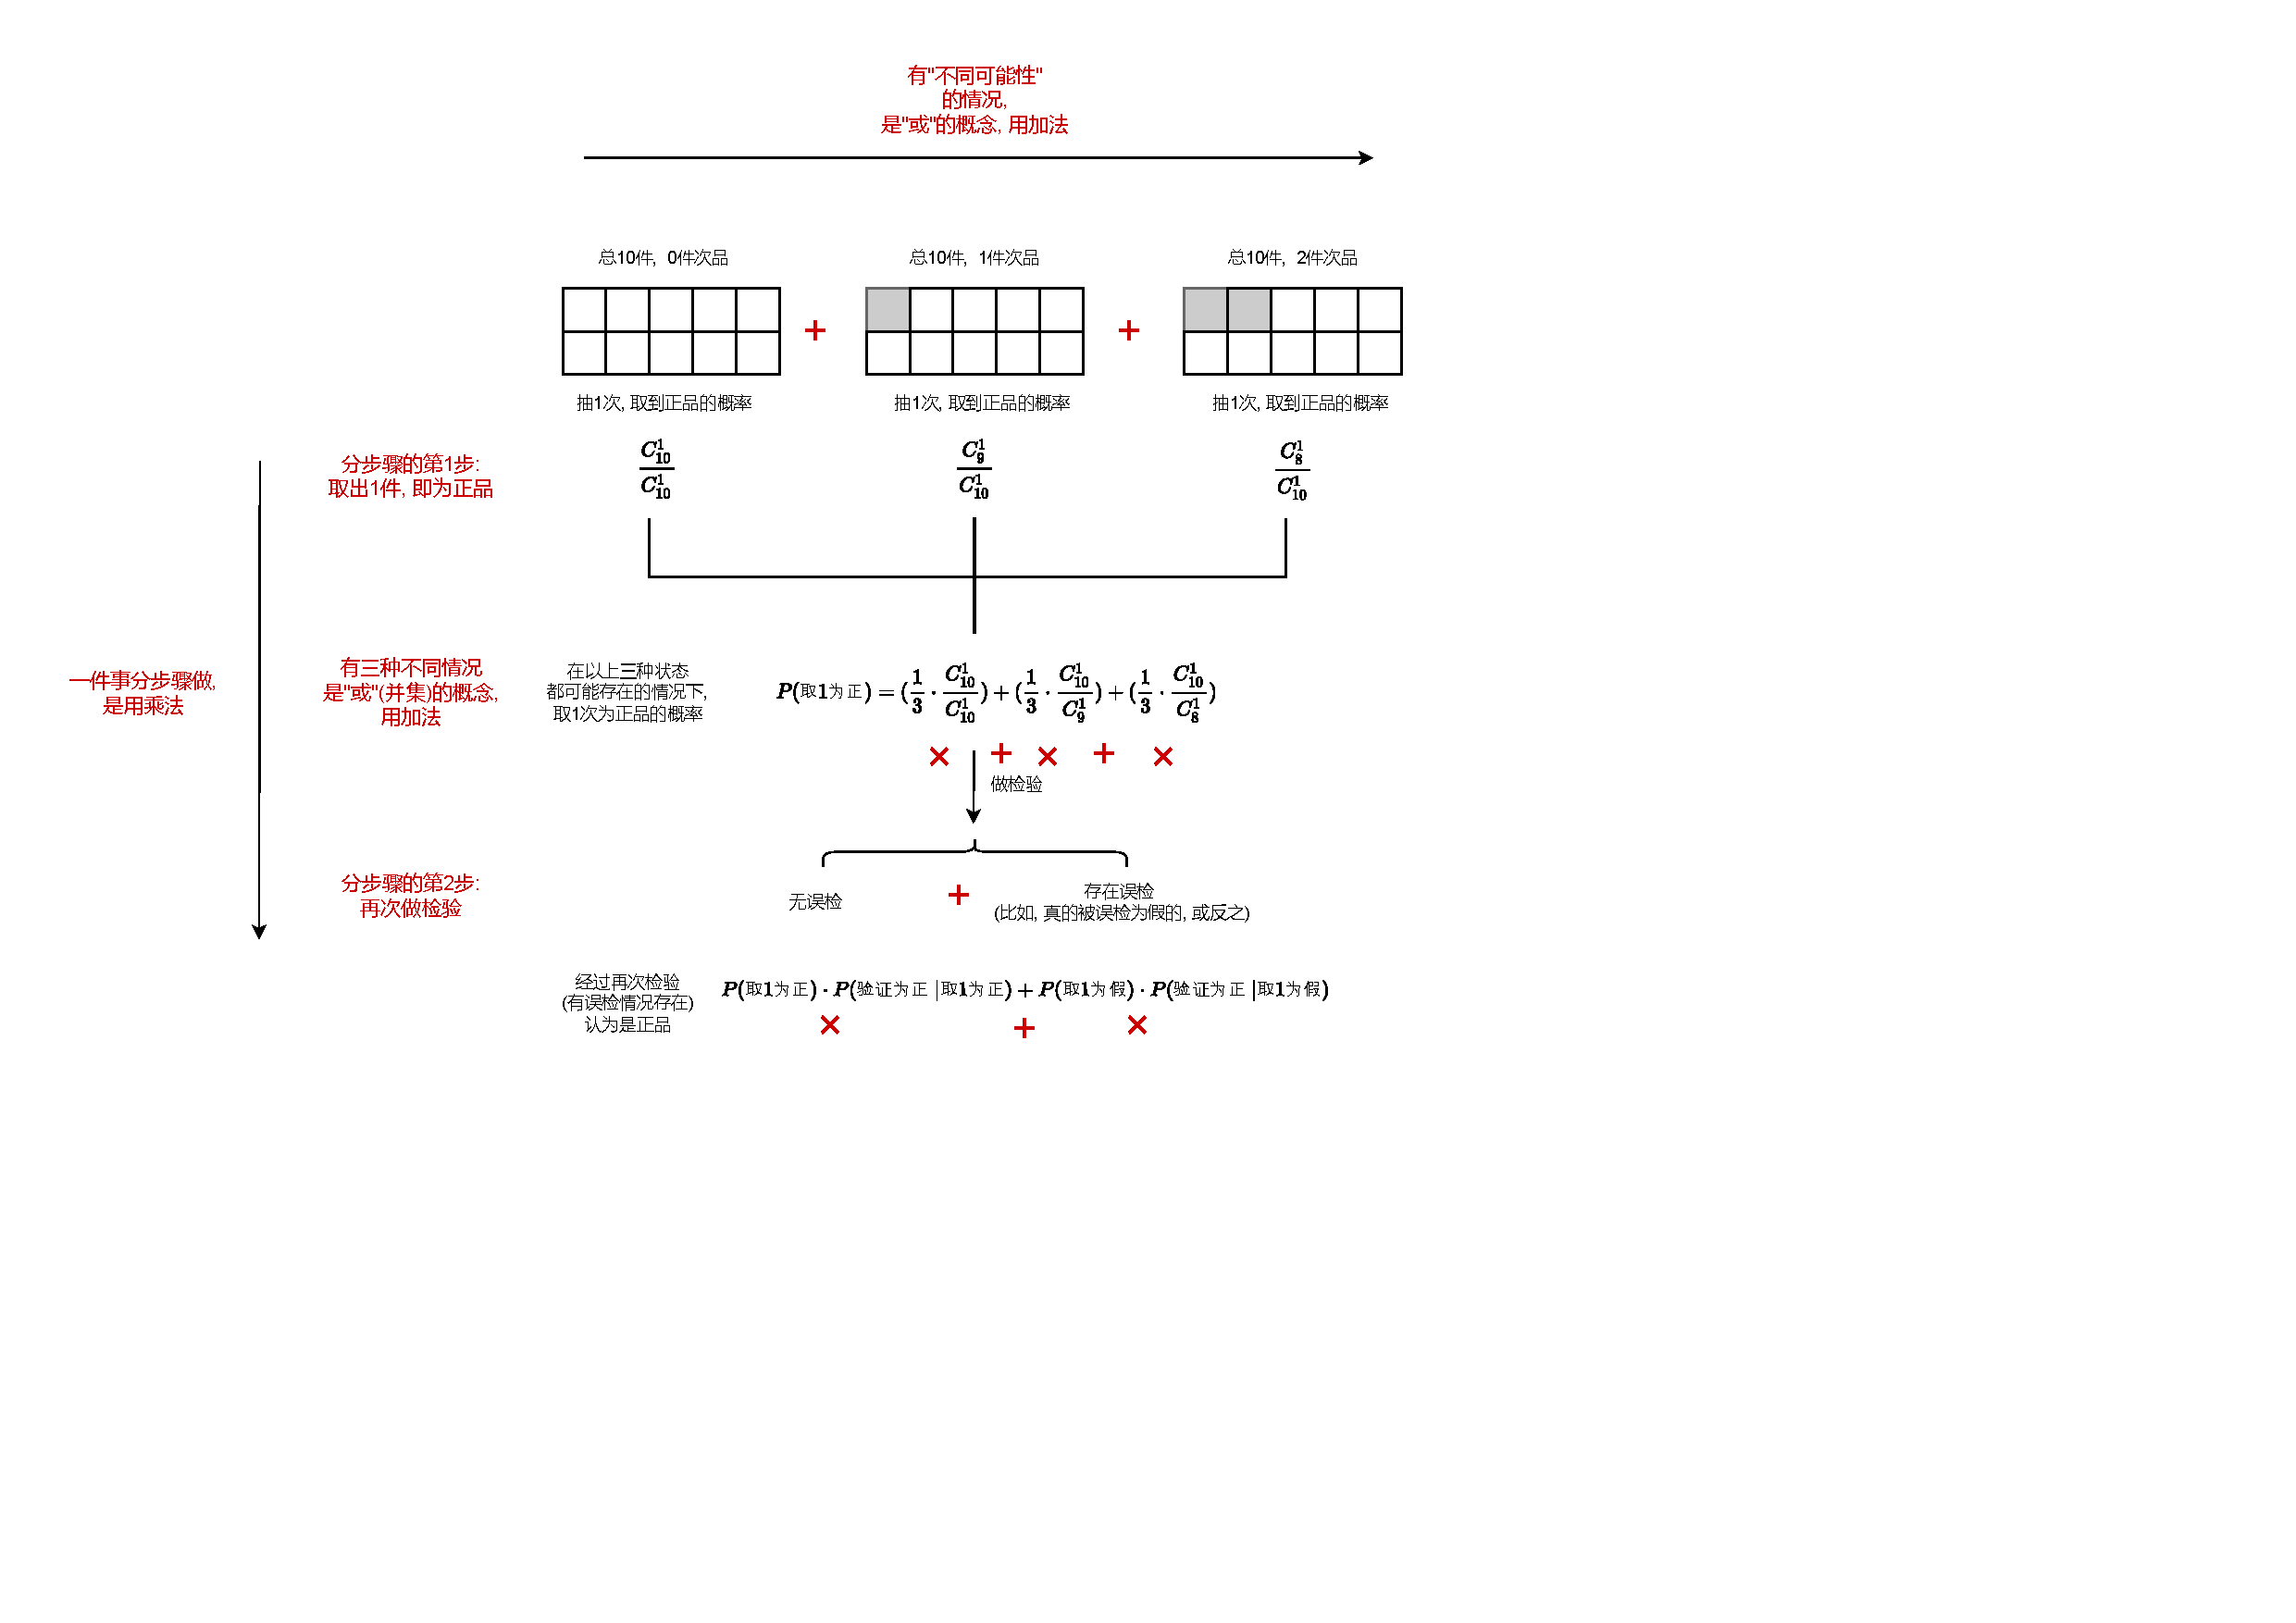
\includegraphics[width=1\textwidth]{/0098.pdf}
	\end{myEnvSample}
	

	
	
	
\end{document}